%%%%%%%%%%%%%%%%%%%%%%%%%%%%%%%%%%%%%%%%%
% Structured General Purpose Assignment
% LaTeX Template
%
% This template has been downloaded from:
% http://www.latextemplates.com
%
% Original author:
% Ted Pavlic (http://www.tedpavlic.com)
%
% Note:
% The \lipsum[#] commands throughout this template generate dummy text
% to fill the template out. These commands should all be removed when 
% writing assignment content.
%
%%%%%%%%%%%%%%%%%%%%%%%%%%%%%%%%%%%%%%%%%

%----------------------------------------------------------------------------------------
%   PACKAGES AND OTHER DOCUMENT CONFIGURATIONS
%----------------------------------------------------------------------------------------

\documentclass{article}

\usepackage{fancyhdr} % Required for custom headers
\usepackage{lastpage} % Required to determine the last page for the footer
\usepackage{extramarks} % Required for headers and footers
\usepackage{graphicx} % Required to insert images
\usepackage{lipsum} % Used for inserting dummy 'Lorem ipsum' text into the template
\usepackage{amsmath}
\usepackage{xcolor}
\usepackage{listings}
\usepackage[toc,page]{appendix}
\usepackage{algorithm}
\usepackage{algorithmic}

% Margins
\topmargin=-0.45in
\evensidemargin=0in
\oddsidemargin=0in
\textwidth=6.5in
\textheight=9.0in
\headsep=0.25in 

\linespread{1.1} % Line spacing

% Set up the header and footer
\pagestyle{fancy}
\lhead{\hmwkAuthorName} % Top left header
\chead{\hmwkClass\ (\hmwkClassInstructor): \hmwkTitle} % Top center header
\rhead{\firstxmark} % Top right header
\lfoot{\lastxmark} % Bottom left footer
\cfoot{} % Bottom center footer
\rfoot{Page\ \thepage\ of\ \pageref{LastPage}} % Bottom right footer
\renewcommand\headrulewidth{0.4pt} % Size of the header rule
\renewcommand\footrulewidth{0.4pt} % Size of the footer rule

\setlength\parindent{0pt} % Removes all indentation from paragraphs

%----------------------------------------------------------------------------------------
%   DOCUMENT STRUCTURE COMMANDS
%   Skip this unless you know what you're doing
%----------------------------------------------------------------------------------------

% Header and footer for when a page split occurs within a problem environment
\newcommand{\enterProblemHeader}[1]{
    \nobreak\extramarks{#1}{#1 continued on next page\ldots}\nobreak
    \nobreak\extramarks{#1 (continued)}{#1 continued on next page\ldots}\nobreak
}

% Header and footer for when a page split occurs between problem environments
\newcommand{\exitProblemHeader}[1]{
    \nobreak\extramarks{#1 (continued)}{#1 continued on next page\ldots}\nobreak
    \nobreak\extramarks{#1}{}\nobreak
}

\setcounter{secnumdepth}{0} % Removes default section numbers
\newcounter{homeworkProblemCounter} % Creates a counter to keep track of the number of problems
\setcounter{homeworkProblemCounter}{0}

\newcommand{\homeworkProblemName}{}
\newenvironment{homeworkProblem}[1][Problem \arabic{homeworkProblemCounter}]{ % Makes a new environment called homeworkProblem which takes 1 argument (custom name) but the default is "Problem #"
    \stepcounter{homeworkProblemCounter} % Increase counter for number of
% problems
    \renewcommand{\homeworkProblemName}{#1} % Assign \homeworkProblemName the
% name of the problem
    \section{\homeworkProblemName} % Make a section in the document with the
% custom problem count
    \enterProblemHeader{\homeworkProblemName} % Header and footer within the
% environment
}{
    \exitProblemHeader{\homeworkProblemName} % Header and footer after the
% environment
}

\newcommand{\problemAnswer}[1]{ % Defines the problem answer command with the content as the only argument
    \noindent\textbf{\emph{Answer: }}#1 % Just put a keyword Answer in
    % bold/italic at the beginning
}

\newcommand{\homeworkSectionName}{}
\newenvironment{homeworkSection}[1]{ % New environment for sections within homework problems, takes 1 argument - the name of the section
    \renewcommand{\homeworkSectionName}{#1} % Assign \homeworkSectionName to the
% name of the section from the environment argument
    \subsection{\homeworkSectionName} % Make a subsection with the custom name
% of the subsection
    \enterProblemHeader{\homeworkProblemName\ [\homeworkSectionName]} % Header
% and footer within the environment
}{
    \enterProblemHeader{\homeworkProblemName} % Header and footer after the
% environment
}

\newtheorem{theorem}{Theorem}[homeworkProblemCounter]
\newtheorem{lemma}[theorem]{Lemma}
\newtheorem{proposition}[theorem]{Proposition}
\newtheorem{corollary}[theorem]{Corollary}

\newenvironment{proof}[1][Proof]{
    \begin{trivlist}
        \item[\hskip \labelsep {\bfseries #1}]
    }{
        \end{trivlist}
}
\newenvironment{definition}[1][Definition]{
    \begin{trivlist}
        \item[\hskip \labelsep {\bfseries #1}]
    }{
        \end{trivlist}
}
\newenvironment{example}[1][Example]{
    \begin{trivlist}
        \item[\hskip \labelsep {\bfseries #1}]
    }{
        \end{trivlist}
    }
\newenvironment{remark}[1][Remark]{
    \begin{trivlist}
        \item[\hskip \labelsep {\bfseries #1}]
    }{
        \end{trivlist}
}

\newcommand{\qed}{
    \nobreak \ifvmode \relax \else
    \ifdim\lastskip<1.5em \hskip-\lastskip
    \hskip1.5em plus0em minus0.5em \fi \nobreak
    \vrule height0.75em width0.5em depth0.25em\fi
}

\lstset{
    frame=single,
    breaklines=true,
    postbreak=\raisebox{0ex}[0ex][0ex]{\ensuremath{\color{red}\hookrightarrow\space}}
}
   
%----------------------------------------------------------------------------------------
%   NAME AND CLASS SECTION
%----------------------------------------------------------------------------------------

\newcommand{\hmwkTitle}{Assignment\ \#4} % Assignment title
\newcommand{\hmwkDueDate}{Tuesday,February\ 12,\ 2015} % Due date
\newcommand{\hmwkClass}{ECS\ 222A} % Course/class
\newcommand{\hmwkClassTime}{TR 4:40pm-6:00pm} % Class/lecture time
\newcommand{\hmwkClassInstructor}{Daniel Gusfield} % Teacher/lecturer
\newcommand{\hmwkAuthorName}{Wenhao Wu} % Your name

%----------------------------------------------------------------------------------------
%   TITLE PAGE
%----------------------------------------------------------------------------------------

\title{
    \vspace{2in}
    \textmd{\textbf{\hmwkClass:\ \hmwkTitle}}\\
    \normalsize\vspace{0.1in}\small{Due\ on\ \hmwkDueDate}\\
    \vspace{0.1in}\large{\textit{\hmwkClassInstructor\ \hmwkClassTime}}
    \vspace{3in}
}

\author{\textbf{\hmwkAuthorName}}
\date{} % Insert date here if you want it to appear below your name

%----------------------------------------------------------------------------------------

\begin{document}

    \maketitle
    
    %----------------------------------------------------------------------------------------
    %   TABLE OF CONTENTS
    %----------------------------------------------------------------------------------------
    
    %\setcounter{tocdepth}{1} % Uncomment this line if you don't want subsections listed in the ToC
    
    \newpage
    \tableofcontents
    \newpage

    %----------------------------------------------------------------------------------------
    %   PROBLEM 1
    %----------------------------------------------------------------------------------------
    \begin{homeworkProblem}
        \textbf{(The bipartite node cover problem)} Let $G$ be an undirected
        graph with each node $i$ given weight $w(i) > 0$. A set of nodes $S$ is
        a \emph{node cover} of $G$ if every edge of $G$ is incident to at least
        one node of $S$. The weight of a node cover $S$ is the summation of the
        weights, denoted $w(S)$, of the nodes in $S$; the weighted node cover
        problem is to select a node cover with \emph{minimum weight}.
        \\\\
        There is no known polynomial time (in terms of worst case) algorithm for
        the node cover problem (even when all weights are one). But if $G$ is
        bipartite, then the minimum weight node cover can be found in polynomial
        time by network flow. If you don’t know what a bipartite graph is, look
        up a definition in the book.
        \\\\
        Explain how to do this. Hint: Use maximum flow, but the minimun cut is
        the key, rather than the maximum flow.
        
        \vspace{10pt}
        \problemAnswer{
                
         }
        
    \end{homeworkProblem}
    
    %----------------------------------------------------------------------------------------
    %   PROBLEM 2
    %----------------------------------------------------------------------------------------
    \begin{homeworkProblem}
        First, read Section 7.7 in the book to learn about circulations and
        maximum flow with lower bounds on edge flows. Then use what you have
        learned to solve the following problem. You must use network flow with
        lower bounds, even if you see another solution method.
        \\\\
        \textbf{(Table Rounding problem)} You are given an $n$ by $m$ table of
        numbers between 0 and 1 along with row and column totals. Your objective
        is to round each entry to either 0 or 1 (you have complete freedom in
        this) so that each resulting row and column total is itself rounded to
        one of its \emph{two} nearest integers, and so that the table total is
        rounded to one of its two nearest integers. However, any number which
        was originally an integer must not change. For example,
        
        \begin{figure}[!h]
            \centering
            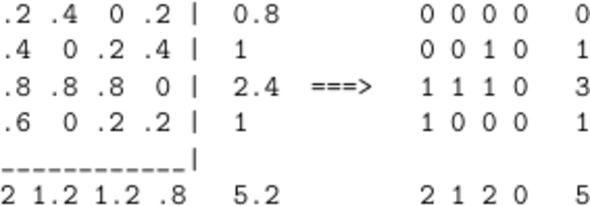
\includegraphics[width=0.5\columnwidth]{figs/table_rounding.pdf}
            \caption{A table rounding examples.}
            \label{fig:table_rounding}
        \end{figure}
        
        Give an efficient algorithm, using network flow, that always finds such
        a rounding. This also provides a proof that such a rounding is always
        possible.
        
        \vspace{10pt}
        \problemAnswer{
                
        }
        
    \end{homeworkProblem}
    
    %----------------------------------------------------------------------------------------
    %   PROBLEM 3
    %----------------------------------------------------------------------------------------
    \begin{homeworkProblem}
        Suppose $(X, Y)$ and $(X', Y')$ are two distinct minimum-capacity $s$,
        $t$ cuts in a directed network $G$. Prove that $(X\cup X' , Y\cup Y')$
        and $(X\cap X , Y\cap Y)$ are also a minimum-capacity $s$, $t$ cuts in
        $G$. The key to this problem is to remember that an $s$, $t$ cut is a
        partition of the nodes with $s$ in one subset and $t$ in the other, so
        there are four subsets of nodes when you examine $X$, $Y$, $X'$, $Y'$
        together; then do a case analysis by looking closely at the capacities
        of the edges from one subset of nodes to another.
        
        \vspace{10pt}
        \problemAnswer{
            
        }
    \end{homeworkProblem}
    %\clearpage
    
    %----------------------------------------------------------------------------------------
    %   PROBLEM 4
    %----------------------------------------------------------------------------------------
    \begin{homeworkProblem}
         In some applications of numerical linear algebra you are given a sparse
         square matrix $M$ (say $n$ by $n$) and you want to permute the rows and
         columns of $M$ so that the main diagonal has no 0, if possible. Show
         how to find such a permutation, if there is one, by using network flow.
         Hint: The key here is to use network flow to find a set of $n$ non-zero
         entries in $M$ such that no two are in the same row or column. For the
         network, start with a bipartite graph to represent the non-zero
         entries of $M$, and then add the $s$ and $t$ nodes.
        
        
        \vspace{10pt}
        \problemAnswer{
                
                
        }
     
    \end{homeworkProblem}
    %\clearpage
    
    %----------------------------------------------------------------------------------------
    %   PROBLEM 5
    %----------------------------------------------------------------------------------------
    \begin{homeworkProblem}
        
         Show that if $f$ is some non-maximum $s-t$ flow in a graph $G$, and
         $G_f$ is the residual graph with respect to $f$, then flow $f$
         \emph{superimposed} with a maximum $s-t$ flow $g$ in $G_f$ is a maximum
         flow in $G$. By superposition we mean the addition of the two flows;
         however if for an edge $(i,j)$ there is flow from $i$ to $j$ in $f$ and
         flow from $j$ to $i$ in $g$ (recall that $g$ is a flow in $G_f$ so that
         this is possible, since $(j,i)$ is a backward edge) then the
         superposition of these flows means the subtraction of $g(j,i)$ from
         $f(i,j)$. That is, forward flows in $f$ and $g$ are added, but a
         backward flow in $g$ is subtracted from the corresponding forward flow
         in $f$.
        
        \vspace{10pt}
        \problemAnswer{
                
        }
     
    \end{homeworkProblem}
    %\clearpage
    
    %----------------------------------------------------------------------------------------

\end{document}